
%% bare_adv.tex
%% V1.4b
%% 2015/08/26
%% by Michael Shell
%% See: 
%% http://www.michaelshell.org/
%% for current contact information.
%%
%% This is a skeleton file demonstrating the advanced use of IEEEtran.cls
%% (requires IEEEtran.cls version 1.8b or later) with an IEEE Computer
%% Society journal paper.
%%
%% Support sites:
%% http://www.michaelshell.org/tex/ieeetran/
%% http://www.ctan.org/pkg/ieeetran
%% and
%% http://www.ieee.org/

%%*************************************************************************
%% Legal Notice:
%% This code is offered as-is without any warranty either expressed or
%% implied; without even the implied warranty of MERCHANTABILITY or
%% FITNESS FOR A PARTICULAR PURPOSE! 
%% User assumes all risk.
%% In no event shall the IEEE or any contributor to this code be liable for
%% any damages or losses, including, but not limited to, incidental,
%% consequential, or any other damages, resulting from the use or misuse
%% of any information contained here.
%%
%% All comments are the opinions of their respective authors and are not
%% necessarily endorsed by the IEEE.
%%
%% This work is distributed under the LaTeX Project Public License (LPPL)
%% ( http://www.latex-project.org/ ) version 1.3, and may be freely used,
%% distributed and modified. A copy of the LPPL, version 1.3, is included
%% in the base LaTeX documentation of all distributions of LaTeX released
%% 2003/12/01 or later.
%% Retain all contribution notices and credits.
%% ** Modified files should be clearly indicated as such, including  **
%% ** renaming them and changing author support contact information. **
%%*************************************************************************


% *** Authors should verify (and, if needed, correct) their LaTeX system  ***
% *** with the testflow diagnostic prior to trusting their LaTeX platform ***
% *** with production work. The IEEE's font choices and paper sizes can   ***
% *** trigger bugs that do not appear when using other class files.       ***                          ***
% The testflow support page is at:
% http://www.michaelshell.org/tex/testflow/


% IEEEtran V1.7 and later provides for these CLASSINPUT macros to allow the
% user to reprogram some IEEEtran.cls defaults if needed. These settings
% override the internal defaults of IEEEtran.cls regardless of which class
% options are used. Do not use these unless you have good reason to do so as
% they can result in nonIEEE compliant documents. User beware. ;)
%
%\newcommand{\CLASSINPUTbaselinestretch}{1.0} % baselinestretch
%\newcommand{\CLASSINPUTinnersidemargin}{1in} % inner side margin
%\newcommand{\CLASSINPUToutersidemargin}{1in} % outer side margin
%\newcommand{\CLASSINPUTtoptextmargin}{1in}   % top text margin
%\newcommand{\CLASSINPUTbottomtextmargin}{1in}% bottom text margin




%
\documentclass[10pt,journal,compsoc]{IEEEtran}
% If IEEEtran.cls has not been installed into the LaTeX system files,
% manually specify the path to it like:
% \documentclass[10pt,journal,compsoc]{../sty/IEEEtran}

\usepackage{graphicx}
\usepackage{amsmath}
\usepackage{hyperref}
% For Computer Society journals, IEEEtran defaults to the use of 
% Palatino/Palladio as is done in IEEE Computer Society journals.
% To go back to Times Roman, you can use this code:
%\renewcommand{\rmdefault}{ptm}\selectfont





% Some very useful LaTeX packages include:
% (uncomment the ones you want to load)



% *** MISC UTILITY PACKAGES ***
%
%\usepackage{ifpdf}
% Heiko Oberdiek's ifpdf.sty is very useful if you need conditional
% compilation based on whether the output is pdf or dvi.
% usage:
% \ifpdf
%   % pdf code
% \else
%   % dvi code
% \fi
% The latest version of ifpdf.sty can be obtained from:
% http://www.ctan.org/pkg/ifpdf
% Also, note that IEEEtran.cls V1.7 and later provides a builtin
% \ifCLASSINFOpdf conditional that works the same way.
% When switching from latex to pdflatex and vice-versa, the compiler may
% have to be run twice to clear warning/error messages.






% *** CITATION PACKAGES ***
%
\ifCLASSOPTIONcompsoc
  % The IEEE Computer Society needs nocompress option
  % requires cite.sty v4.0 or later (November 2003)
  \usepackage[nocompress]{cite}
\else
  % normal IEEE
  \usepackage{cite}
\fi
% cite.sty was written by Donald Arseneau
% V1.6 and later of IEEEtran pre-defines the format of the cite.sty package
% \cite{} output to follow that of the IEEE. Loading the cite package will
% result in citation numbers being automatically sorted and properly
% "compressed/ranged". e.g., [1], [9], [2], [7], [5], [6] without using
% cite.sty will become [1], [2], [5]--[7], [9] using cite.sty. cite.sty's
% \cite will automatically add leading space, if needed. Use cite.sty's
% noadjust option (cite.sty V3.8 and later) if you want to turn this off
% such as if a citation ever needs to be enclosed in parenthesis.
% cite.sty is already installed on most LaTeX systems. Be sure and use
% version 5.0 (2009-03-20) and later if using hyperref.sty.
% The latest version can be obtained at:
% http://www.ctan.org/pkg/cite
% The documentation is contained in the cite.sty file itself.
%
% Note that some packages require special options to format as the Computer
% Society requires. In particular, Computer Society  papers do not use
% compressed citation ranges as is done in typical IEEE papers
% (e.g., [1]-[4]). Instead, they list every citation separately in order
% (e.g., [1], [2], [3], [4]). To get the latter we need to load the cite
% package with the nocompress option which is supported by cite.sty v4.0
% and later.





% *** GRAPHICS RELATED PACKAGES ***
%
\ifCLASSINFOpdf
  % \usepackage[pdftex]{graphicx}
  % declare the path(s) where your graphic files are
  % \graphicspath{{../pdf/}{../jpeg/}}
  % and their extensions so you won't have to specify these with
  % every instance of \includegraphics
  % \DeclareGraphicsExtensions{.pdf,.jpeg,.png}
\else
  % or other class option (dvipsone, dvipdf, if not using dvips). graphicx
  % will default to the driver specified in the system graphics.cfg if no
  % driver is specified.
  % \usepackage[dvips]{graphicx}
  % declare the path(s) where your graphic files are
  % \graphicspath{{../eps/}}
  % and their extensions so you won't have to specify these with
  % every instance of \includegraphics
  % \DeclareGraphicsExtensions{.eps}
\fi
% graphicx was written by David Carlisle and Sebastian Rahtz. It is
% required if you want graphics, photos, etc. graphicx.sty is already
% installed on most LaTeX systems. The latest version and documentation
% can be obtained at: 
% http://www.ctan.org/pkg/graphicx
% Another good source of documentation is "Using Imported Graphics in
% LaTeX2e" by Keith Reckdahl which can be found at:
% http://www.ctan.org/pkg/epslatex
%
% latex, and pdflatex in dvi mode, support graphics in encapsulated
% postscript (.eps) format. pdflatex in pdf mode supports graphics
% in .pdf, .jpeg, .png and .mps (metapost) formats. Users should ensure
% that all non-photo figures use a vector format (.eps, .pdf, .mps) and
% not a bitmapped formats (.jpeg, .png). The IEEE frowns on bitmapped formats
% which can result in "jaggedy"/blurry rendering of lines and letters as
% well as large increases in file sizes.
%
% You can find documentation about the pdfTeX application at:
% http://www.tug.org/applications/pdftex





% *** MATH PACKAGES ***
%
%\usepackage{amsmath}
% A popular package from the American Mathematical Society that provides
% many useful and powerful commands for dealing with mathematics.
%
% Note that the amsmath package sets \interdisplaylinepenalty to 10000
% thus preventing page breaks from occurring within multiline equations. Use:
%\interdisplaylinepenalty=2500
% after loading amsmath to restore such page breaks as IEEEtran.cls normally
% does. amsmath.sty is already installed on most LaTeX systems. The latest
% version and documentation can be obtained at:
% http://www.ctan.org/pkg/amsmath





% *** SPECIALIZED LIST PACKAGES ***
%\usepackage{acronym}
% acronym.sty was written by Tobias Oetiker. This package provides tools for
% managing documents with large numbers of acronyms. (You don't *have* to
% use this package - unless you have a lot of acronyms, you may feel that
% such package management of them is bit of an overkill.)
% Do note that the acronym environment (which lists acronyms) will have a
% problem when used under IEEEtran.cls because acronym.sty relies on the
% description list environment - which IEEEtran.cls has customized for
% producing IEEE style lists. A workaround is to declared the longest
% label width via the IEEEtran.cls \IEEEiedlistdecl global control:
%
% \renewcommand{\IEEEiedlistdecl}{\IEEEsetlabelwidth{SONET}}
% \begin{acronym}
%
% \end{acronym}
% \renewcommand{\IEEEiedlistdecl}{\relax}% remember to reset \IEEEiedlistdecl
%
% instead of using the acronym environment's optional argument.
% The latest version and documentation can be obtained at:
% http://www.ctan.org/pkg/acronym


%\usepackage{algorithmic}
% algorithmic.sty was written by Peter Williams and Rogerio Brito.
% This package provides an algorithmic environment fo describing algorithms.
% You can use the algorithmic environment in-text or within a figure
% environment to provide for a floating algorithm. Do NOT use the algorithm
% floating environment provided by algorithm.sty (by the same authors) or
% algorithm2e.sty (by Christophe Fiorio) as the IEEE does not use dedicated
% algorithm float types and packages that provide these will not provide
% correct IEEE style captions. The latest version and documentation of
% algorithmic.sty can be obtained at:
% http://www.ctan.org/pkg/algorithms
% Also of interest may be the (relatively newer and more customizable)
% algorithmicx.sty package by Szasz Janos:
% http://www.ctan.org/pkg/algorithmicx




% *** ALIGNMENT PACKAGES ***
%
%\usepackage{array}
% Frank Mittelbach's and David Carlisle's array.sty patches and improves
% the standard LaTeX2e array and tabular environments to provide better
% appearance and additional user controls. As the default LaTeX2e table
% generation code is lacking to the point of almost being broken with
% respect to the quality of the end results, all users are strongly
% advised to use an enhanced (at the very least that provided by array.sty)
% set of table tools. array.sty is already installed on most systems. The
% latest version and documentation can be obtained at:
% http://www.ctan.org/pkg/array


%\usepackage{mdwmath}
%\usepackage{mdwtab}
% Also highly recommended is Mark Wooding's extremely powerful MDW tools,
% especially mdwmath.sty and mdwtab.sty which are used to format equations
% and tables, respectively. The MDWtools set is already installed on most
% LaTeX systems. The lastest version and documentation is available at:
% http://www.ctan.org/pkg/mdwtools


% IEEEtran contains the IEEEeqnarray family of commands that can be used to
% generate multiline equations as well as matrices, tables, etc., of high
% quality.


%\usepackage{eqparbox}
% Also of notable interest is Scott Pakin's eqparbox package for creating
% (automatically sized) equal width boxes - aka "natural width parboxes".
% Available at:
% http://www.ctan.org/pkg/eqparbox




% *** SUBFIGURE PACKAGES ***
%\ifCLASSOPTIONcompsoc
%  \usepackage[caption=false,font=footnotesize,labelfont=sf,textfont=sf]{subfig}
%\else
%  \usepackage[caption=false,font=footnotesize]{subfig}
%\fi
% subfig.sty, written by Steven Douglas Cochran, is the modern replacement
% for subfigure.sty, the latter of which is no longer maintained and is
% incompatible with some LaTeX packages including fixltx2e. However,
% subfig.sty requires and automatically loads Axel Sommerfeldt's caption.sty
% which will override IEEEtran.cls' handling of captions and this will result
% in non-IEEE style figure/table captions. To prevent this problem, be sure
% and invoke subfig.sty's "caption=false" package option (available since
% subfig.sty version 1.3, 2005/06/28) as this is will preserve IEEEtran.cls
% handling of captions.
% Note that the Computer Society format requires a sans serif font rather
% than the serif font used in traditional IEEE formatting and thus the need
% to invoke different subfig.sty package options depending on whether
% compsoc mode has been enabled.
%
% The latest version and documentation of subfig.sty can be obtained at:
% http://www.ctan.org/pkg/subfig




% *** FLOAT PACKAGES ***
%
%\usepackage{fixltx2e}
% fixltx2e, the successor to the earlier fix2col.sty, was written by
% Frank Mittelbach and David Carlisle. This package corrects a few problems
% in the LaTeX2e kernel, the most notable of which is that in current
% LaTeX2e releases, the ordering of single and double column floats is not
% guaranteed to be preserved. Thus, an unpatched LaTeX2e can allow a
% single column figure to be placed prior to an earlier double column
% figure.
% Be aware that LaTeX2e kernels dated 2015 and later have fixltx2e.sty's
% corrections already built into the system in which case a warning will
% be issued if an attempt is made to load fixltx2e.sty as it is no longer
% needed.
% The latest version and documentation can be found at:
% http://www.ctan.org/pkg/fixltx2e


%\usepackage{stfloats}
% stfloats.sty was written by Sigitas Tolusis. This package gives LaTeX2e
% the ability to do double column floats at the bottom of the page as well
% as the top. (e.g., "\begin{figure*}[!b]" is not normally possible in
% LaTeX2e). It also provides a command:
%\fnbelowfloat
% to enable the placement of footnotes below bottom floats (the standard
% LaTeX2e kernel puts them above bottom floats). This is an invasive package
% which rewrites many portions of the LaTeX2e float routines. It may not work
% with other packages that modify the LaTeX2e float routines. The latest
% version and documentation can be obtained at:
% http://www.ctan.org/pkg/stfloats
% Do not use the stfloats baselinefloat ability as the IEEE does not allow
% \baselineskip to stretch. Authors submitting work to the IEEE should note
% that the IEEE rarely uses double column equations and that authors should try
% to avoid such use. Do not be tempted to use the cuted.sty or midfloat.sty
% packages (also by Sigitas Tolusis) as the IEEE does not format its papers in
% such ways.
% Do not attempt to use stfloats with fixltx2e as they are incompatible.
% Instead, use Morten Hogholm'a dblfloatfix which combines the features
% of both fixltx2e and stfloats:
%
% \usepackage{dblfloatfix}
% The latest version can be found at:
% http://www.ctan.org/pkg/dblfloatfix


%\ifCLASSOPTIONcaptionsoff
%  \usepackage[nomarkers]{endfloat}
% \let\MYoriglatexcaption\caption
% \renewcommand{\caption}[2][\relax]{\MYoriglatexcaption[#2]{#2}}
%\fi
% endfloat.sty was written by James Darrell McCauley, Jeff Goldberg and 
% Axel Sommerfeldt. This package may be useful when used in conjunction with 
% IEEEtran.cls'  captionsoff option. Some IEEE journals/societies require that
% submissions have lists of figures/tables at the end of the paper and that
% figures/tables without any captions are placed on a page by themselves at
% the end of the document. If needed, the draftcls IEEEtran class option or
% \CLASSINPUTbaselinestretch interface can be used to increase the line
% spacing as well. Be sure and use the nomarkers option of endfloat to
% prevent endfloat from "marking" where the figures would have been placed
% in the text. The two hack lines of code above are a slight modification of
% that suggested by in the endfloat docs (section 8.4.1) to ensure that
% the full captions always appear in the list of figures/tables - even if
% the user used the short optional argument of \caption[]{}.
% IEEE papers do not typically make use of \caption[]'s optional argument,
% so this should not be an issue. A similar trick can be used to disable
% captions of packages such as subfig.sty that lack options to turn off
% the subcaptions:
% For subfig.sty:
% \let\MYorigsubfloat\subfloat
% \renewcommand{\subfloat}[2][\relax]{\MYorigsubfloat[]{#2}}
% However, the above trick will not work if both optional arguments of
% the \subfloat command are used. Furthermore, there needs to be a
% description of each subfigure *somewhere* and endfloat does not add
% subfigure captions to its list of figures. Thus, the best approach is to
% avoid the use of subfigure captions (many IEEE journals avoid them anyway)
% and instead reference/explain all the subfigures within the main caption.
% The latest version of endfloat.sty and its documentation can obtained at:
% http://www.ctan.org/pkg/endfloat
%
% The IEEEtran \ifCLASSOPTIONcaptionsoff conditional can also be used
% later in the document, say, to conditionally put the References on a 
% page by themselves.





% *** PDF, URL AND HYPERLINK PACKAGES ***
%
%\usepackage{url}
% url.sty was written by Donald Arseneau. It provides better support for
% handling and breaking URLs. url.sty is already installed on most LaTeX
% systems. The latest version and documentation can be obtained at:
% http://www.ctan.org/pkg/url
% Basically, \url{my_url_here}.


% NOTE: PDF thumbnail features are not required in IEEE papers
%       and their use requires extra complexity and work.
%\ifCLASSINFOpdf
%  \usepackage[pdftex]{thumbpdf}
%\else
%  \usepackage[dvips]{thumbpdf}
%\fi
% thumbpdf.sty and its companion Perl utility were written by Heiko Oberdiek.
% It allows the user a way to produce PDF documents that contain fancy
% thumbnail images of each of the pages (which tools like acrobat reader can
% utilize). This is possible even when using dvi->ps->pdf workflow if the
% correct thumbpdf driver options are used. thumbpdf.sty incorporates the
% file containing the PDF thumbnail information (filename.tpm is used with
% dvips, filename.tpt is used with pdftex, where filename is the base name of
% your tex document) into the final ps or pdf output document. An external
% utility, the thumbpdf *Perl script* is needed to make these .tpm or .tpt
% thumbnail files from a .ps or .pdf version of the document (which obviously
% does not yet contain pdf thumbnails). Thus, one does a:
% 
% thumbpdf filename.pdf 
%
% to make a filename.tpt, and:
%
% thumbpdf --mode dvips filename.ps
%
% to make a filename.tpm which will then be loaded into the document by
% thumbpdf.sty the NEXT time the document is compiled (by pdflatex or
% latex->dvips->ps2pdf). Users must be careful to regenerate the .tpt and/or
% .tpm files if the main document changes and then to recompile the
% document to incorporate the revised thumbnails to ensure that thumbnails
% match the actual pages. It is easy to forget to do this!
% 
% Unix systems come with a Perl interpreter. However, MS Windows users
% will usually have to install a Perl interpreter so that the thumbpdf
% script can be run. The Ghostscript PS/PDF interpreter is also required.
% See the thumbpdf docs for details. The latest version and documentation
% can be obtained at.
% http://www.ctan.org/pkg/thumbpdf


% NOTE: PDF hyperlink and bookmark features are not required in IEEE
%       papers and their use requires extra complexity and work.
% *** IF USING HYPERREF BE SURE AND CHANGE THE EXAMPLE PDF ***
% *** TITLE/SUBJECT/AUTHOR/KEYWORDS INFO BELOW!!           ***
\newcommand\MYhyperrefoptions{bookmarks=true,bookmarksnumbered=true,
pdfpagemode={UseOutlines},plainpages=false,pdfpagelabels=true,
colorlinks=true,linkcolor={black},citecolor={black},urlcolor={black},
pdftitle={Bare Demo of IEEEtran.cls for Computer Society Journals},%<!CHANGE!
pdfsubject={Typesetting},%<!CHANGE!
pdfauthor={Michael D. Shell},%<!CHANGE!
pdfkeywords={Computer Society, IEEEtran, journal, LaTeX, paper,
             template}}%<^!CHANGE!
%\ifCLASSINFOpdf
%\usepackage[\MYhyperrefoptions,pdftex]{hyperref}
%\else
%\usepackage[\MYhyperrefoptions,breaklinks=true,dvips]{hyperref}
%\usepackage{breakurl}
%\fi
% One significant drawback of using hyperref under DVI output is that the
% LaTeX compiler cannot break URLs across lines or pages as can be done
% under pdfLaTeX's PDF output via the hyperref pdftex driver. This is
% probably the single most important capability distinction between the
% DVI and PDF output. Perhaps surprisingly, all the other PDF features
% (PDF bookmarks, thumbnails, etc.) can be preserved in
% .tex->.dvi->.ps->.pdf workflow if the respective packages/scripts are
% loaded/invoked with the correct driver options (dvips, etc.). 
% As most IEEE papers use URLs sparingly (mainly in the references), this
% may not be as big an issue as with other publications.
%
% That said, Vilar Camara Neto created his breakurl.sty package which
% permits hyperref to easily break URLs even in dvi mode.
% Note that breakurl, unlike most other packages, must be loaded
% AFTER hyperref. The latest version of breakurl and its documentation can
% be obtained at:
% http://www.ctan.org/pkg/breakurl
% breakurl.sty is not for use under pdflatex pdf mode.
%
% The advanced features offer by hyperref.sty are not required for IEEE
% submission, so users should weigh these features against the added
% complexity of use.
% The package options above demonstrate how to enable PDF bookmarks
% (a type of table of contents viewable in Acrobat Reader) as well as
% PDF document information (title, subject, author and keywords) that is
% viewable in Acrobat reader's Document_Properties menu. PDF document
% information is also used extensively to automate the cataloging of PDF
% documents. The above set of options ensures that hyperlinks will not be
% colored in the text and thus will not be visible in the printed page,
% but will be active on "mouse over". USING COLORS OR OTHER HIGHLIGHTING
% OF HYPERLINKS CAN RESULT IN DOCUMENT REJECTION BY THE IEEE, especially if
% these appear on the "printed" page. IF IN DOUBT, ASK THE RELEVANT
% SUBMISSION EDITOR. You may need to add the option hypertexnames=false if
% you used duplicate equation numbers, etc., but this should not be needed
% in normal IEEE work.
% The latest version of hyperref and its documentation can be obtained at:
% http://www.ctan.org/pkg/hyperref





% *** Do not adjust lengths that control margins, column widths, etc. ***
% *** Do not use packages that alter fonts (such as pslatex).         ***
% There should be no need to do such things with IEEEtran.cls V1.6 and later.
% (Unless specifically asked to do so by the journal or conference you plan
% to submit to, of course. )


% correct bad hyphenation here
\hyphenation{op-tical net-works semi-conduc-tor}


\begin{document}
%
% paper title
% Titles are generally capitalized except for words such as a, an, and, as,
% at, but, by, for, in, nor, of, on, or, the, to and up, which are usually
% not capitalized unless they are the first or last word of the title.
% Linebreaks \\ can be used within to get better formatting as desired.
% Do not put math or special symbols in the title.
\title{Procedural Puzzle Challenge\\
Generation in Fujisan}
%
%
% author names and IEEE memberships
% note positions of commas and nonbreaking spaces ( ~ ) LaTeX will not break
% a structure at a ~ so this keeps an author's name from being broken across
% two lines.
% use \thanks{} to gain access to the first footnote area
% a separate \thanks must be used for each paragraph as LaTeX2e's \thanks
% was not built to handle multiple paragraphs
%
%
%\IEEEcompsocitemizethanks is a special \thanks that produces the bulleted
% lists the Computer Society journals use for "first footnote" author
% affiliations. Use \IEEEcompsocthanksitem which works much like \item
% for each affiliation group. When not in compsoc mode,
% \IEEEcompsocitemizethanks becomes like \thanks and
% \IEEEcompsocthanksitem becomes a line break with idention. This
% facilitates dual compilation, although admittedly the differences in the
% desired content of \author between the different types of papers makes a
% one-size-fits-all approach a daunting prospect. For instance, compsoc 
% journal papers have the author affiliations above the "Manuscript
% received ..."  text while in non-compsoc journals this is reversed. Sigh.

\author{Mark~Goadrich
        and~James~Droscha% <-this % stops a space
\IEEEcompsocitemizethanks{\IEEEcompsocthanksitem M. Goadrich is with the Department
of Mathematics and Computer Science, Hendrix College, Conway,
AR, 72034.\protect\\
% note need leading \protect in front of \\ to get a newline within \thanks as
% \\ is fragile and will error, could use \hfil\break instead.
E-mail: see http://mark.goadrich.com/schedule.html
\IEEEcompsocthanksitem J. Droscha is with Glastyn Games.}% <-this % stops a space
%\thanks{Manuscript received September 30, 2018; revised ???}
}

% note the % following the last \IEEEmembership and also \thanks - 
% these prevent an unwanted space from occurring between the last author name
% and the end of the author line. i.e., if you had this:
% 
% \author{....lastname \thanks{...} \thanks{...} }
%                     ^------------^------------^----Do not want these spaces!
%
% a space would be appended to the last name and could cause every name on that
% line to be shifted left slightly. This is one of those "LaTeX things". For
% instance, "\textbf{A} \textbf{B}" will typeset as "A B" not "AB". To get
% "AB" then you have to do: "\textbf{A}\textbf{B}"
% \thanks is no different in this regard, so shield the last } of each \thanks
% that ends a line with a % and do not let a space in before the next \thanks.
% Spaces after \IEEEmembership other than the last one are OK (and needed) as
% you are supposed to have spaces between the names. For what it is worth,
% this is a minor point as most people would not even notice if the said evil
% space somehow managed to creep in.



% The paper headers
%\markboth{IEEE Transactions on Games,~Vol.~2, No.~1, January~2019}%
\markboth{}%IEEE Transactions on Games,~Vol.~2, No.~1, January~2019}%
{Shell \MakeLowercase{\textit{et al.}}: Bare Advanced Demo of IEEEtran.cls for IEEE Computer Society Journals}
% The only time the second header will appear is for the odd numbered pages
% after the title page when using the twoside option.
% 
% *** Note that you probably will NOT want to include the author's ***
% *** name in the headers of peer review papers.                   ***
% You can use \ifCLASSOPTIONpeerreview for conditional compilation here if
% you desire.



% The publisher's ID mark at the bottom of the page is less important with
% Computer Society journal papers as those publications place the marks
% outside of the main text columns and, therefore, unlike regular IEEE
% journals, the available text space is not reduced by their presence.
% If you want to put a publisher's ID mark on the page you can do it like
% this:
%\IEEEpubid{0000--0000/00\$00.00~\copyright~2015 IEEE}
% or like this to get the Computer Society new two part style.
%\IEEEpubid{\makebox[\columnwidth]{\hfill 0000--0000/00/\$00.00~\copyright~2015 IEEE}%
%\hspace{\columnsep}\makebox[\columnwidth]{Published by the IEEE Computer Society\hfill}}
% Remember, if you use this you must call \IEEEpubidadjcol in the second
% column for its text to clear the IEEEpubid mark (Computer Society journal
% papers don't need this extra clearance.)



% use for special paper notices
%\IEEEspecialpapernotice{(Invited Paper)}



% for Computer Society papers, we must declare the abstract and index terms
% PRIOR to the title within the \IEEEtitleabstractindextext IEEEtran
% command as these need to go into the title area created by \maketitle.
% As a general rule, do not put math, special symbols or citations
% in the abstract or keywords.
\IEEEtitleabstractindextext{%
\begin{abstract}
    Challenges for physical solitaire puzzle games are typically designed in advance by humans and limited in number. Alternately, some games incorporate stochastic setup rules, where the human solver randomly sets up the game board before solving the challenge, which can greatly increase the number of possible challenges. However, these setup rules can often generate unsolvable or uninteresting challenges. To better understand these setup processes, we apply a taxonomy for procedural content generation algorithms to solitaire puzzle games.
    In particular, for the game Fujisan, we examine how different stochastic challenge generation algorithms attempt to minimize undesirable challenges, and we report their affect on ease of physical setup, challenge solvability, and challenge difficulty. We find that algorithms can be simple for the solver yet generate solvable and difficult challenges, by constraining randomness through embedding sub-elements of the puzzle mechanics into the physical pieces of the game.
\end{abstract}

% Note that keywords are not normally used for peerreview papers.
\begin{IEEEkeywords}
Board Games, Procedural Content, Monte Carlo Methods, Game Design
\end{IEEEkeywords}}


% make the title area
\maketitle


% To allow for easy dual compilation without having to reenter the
% abstract/keywords data, the \IEEEtitleabstractindextext text will
% not be used in maketitle, but will appear (i.e., to be "transported")
% here as \IEEEdisplaynontitleabstractindextext when compsoc mode
% is not selected <OR> if conference mode is selected - because compsoc
% conference papers position the abstract like regular (non-compsoc)
% papers do!
\IEEEdisplaynontitleabstractindextext
% \IEEEdisplaynontitleabstractindextext has no effect when using
% compsoc under a non-conference mode.


% For peer review papers, you can put extra information on the cover
% page as needed:
% \ifCLASSOPTIONpeerreview
% \begin{center} \bfseries EDICS Category: 3-BBND \end{center}
% \fi
%
% For peerreview papers, this IEEEtran command inserts a page break and
% creates the second title. It will be ignored for other modes.
\IEEEpeerreviewmaketitle


\ifCLASSOPTIONcompsoc
\IEEEraisesectionheading{\section{Introduction}\label{sec:introduction}}
\else
\section{Introduction}
\label{sec:introduction}
\fi
% Computer Society journal (but not conference!) papers do something unusual
% with the very first section heading (almost always called "Introduction").
% They place it ABOVE the main text! IEEEtran.cls does not automatically do
% this for you, but you can achieve this effect with the provided
% \IEEEraisesectionheading{} command. Note the need to keep any \label that
% is to refer to the section immediately after \section in the above as
% \IEEEraisesectionheading puts \section within a raised box.




% The very first letter is a 2 line initial drop letter followed
% by the rest of the first word in caps (small caps for compsoc).
% 
% form to use if the first word consists of a single letter:
% \IEEEPARstart{A}{demo} file is ....
% 
% form to use if you need the single drop letter followed by
% normal text (unknown if ever used by the IEEE):
% \IEEEPARstart{A}{}demo file is ....
% 
% Some journals put the first two words in caps:
% \IEEEPARstart{T}{his demo} file is ....
% 
% Here we have the typical use of a "T" for an initial drop letter
% and "HIS" in caps to complete the first word.
\IEEEPARstart{F}{ujisan} 
% Maybe start with describing Fujisan, make most of this background section?
\footnote{http://www.ludism.org/ppwiki/Fuji-san} is a physical solitaire puzzle game created for the piecepack game system \cite{GAMESYSTEM}. In this game, a human solver must find a way to cooperatively move four Shinto Priests to the top of Mt. Fuji through incremental steps up the mountainside. A sample Fujisan challenge is shown in Figure \ref{fig:SampleFujisan}, with two Priests on each edge and the goal summit spaces in gray. More details on Fujisan can be found in Section \ref{section:fujisan}.

Challenges for Fujisan are created by the solver, using a random setup process to assemble the game pieces into the mountain. This process naturally leads to three questions. {\it How easy is the setup process for the solver to execute? Can all such challenges be solved? How difficult are the created challenges? }

To answer these questions, we first examine solitaire games through the lens of procedural content generation, where algorithms are used to create game content \cite{PCGSURVEY}. Next, we explore the creation of Fujisan and the piecepack game system for which it was designed. We provide detailed descriptions of five different challenge setup algorithms, then compare and contrast these multiple setup algorithms and constraints using computational simulations. Finally, we evaluate these algorithms with respect to ease of player setup, solvability, and difficulty. We find that algorithms can succeed across all three metrics by carefully incorporating desirable constraints based on the puzzle mechanics of Fujisan. 

%===========================================

\section{Procedural Challenge Generation}  \label{sec:Background}

\noindent
Togelius et al. \cite{SBPCG} describe a general taxonomy of dimensions for characterizing procedural content generation (PCG) algorithms. PCG can occur {\it offline} (beforehand) or {\it online} (dynamically during the game). The content can be {\it constructed}
by a system of rules, or use a {\it generate-and-test} process to winnow potential candidates for inclusion in the game.
The algorithm can be {\it deterministic} and fixed or {\it stochastic}, incorporating randomness.
Finally, the generated content can be {\it necessary} or {\it optional} for playing the game.

\begin{figure}[b]
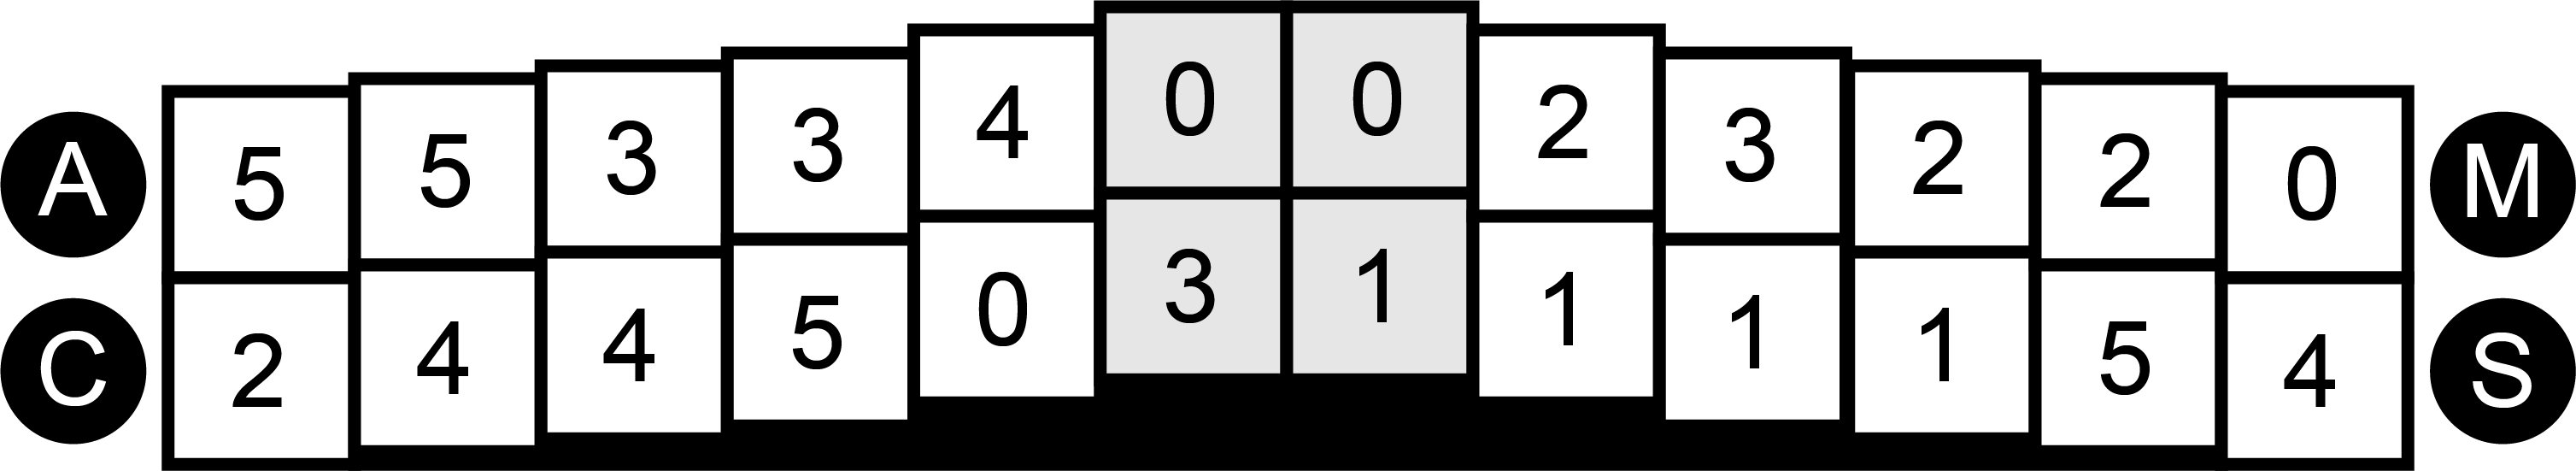
\includegraphics[width=8.8cm]{piecepackexample.png}
\caption{A sample Fujisan puzzle, with the summit denoted in gray.}
\label{fig:SampleFujisan}
\end{figure}



In many ways, the process by which a setter creates a challenge for a particular puzzle can be understood with this PCG taxonomy. We use here the puzzle terminology of Browne \cite{PUZZLENATURE}, such that there is a setter who creates challenges, and a solver who solves them.
For puzzles, setters typically {\it construct} their challenges {\it offline} in advance, using creative yet {\it deterministic} means, and it is {\it necessary} that the challenge be solvable. Researchers have explored using PCG to replace the setter, employing metaheuristics to find interesting challenges for deductive logic puzzles, ranging from Sudoku \cite{SUDOKU} to Nonograms \cite{NONOGRAM}. These algorithms similarly construct their challenges offline, and guarantee they are solvable, but substitute {\it stochastic} algorithms for the creative human process.
Khalifa and Fayek\cite{PUZZLELANG} investigated a combination of construction and generate-and-test PCG for Sokoban challenges within a genetic algorithm framework, and this approach was extended to Monte Carlo Tree Search by Kartal et al. \cite{SOKOBAN}.

A less-explored variety of puzzle with relation to PCG 
are solitaire games, for example
sliding block puzzles \cite{FIFTEEN} (including Rush Hour\footnote{https://www.thinkfun.com/products/rush-hour/}), 
and Hi-Q (generalized peg solitaire) \cite{PEG}. In these games, solvers must manipulate physical pieces to solve a challenge. Since the initial setup for these games must be executed by the solver, providing the solver with predefined challenges and a solution book is common practice. PCG can also be applied to these games by, again, constructing challenges offline and guaranteeing they are solvable, as seen in recent work by Fogleman \cite{RUSHHOUR} and K{\"o}pp \cite{TANGRAM}. 

\begin{figure}[t]
\centering
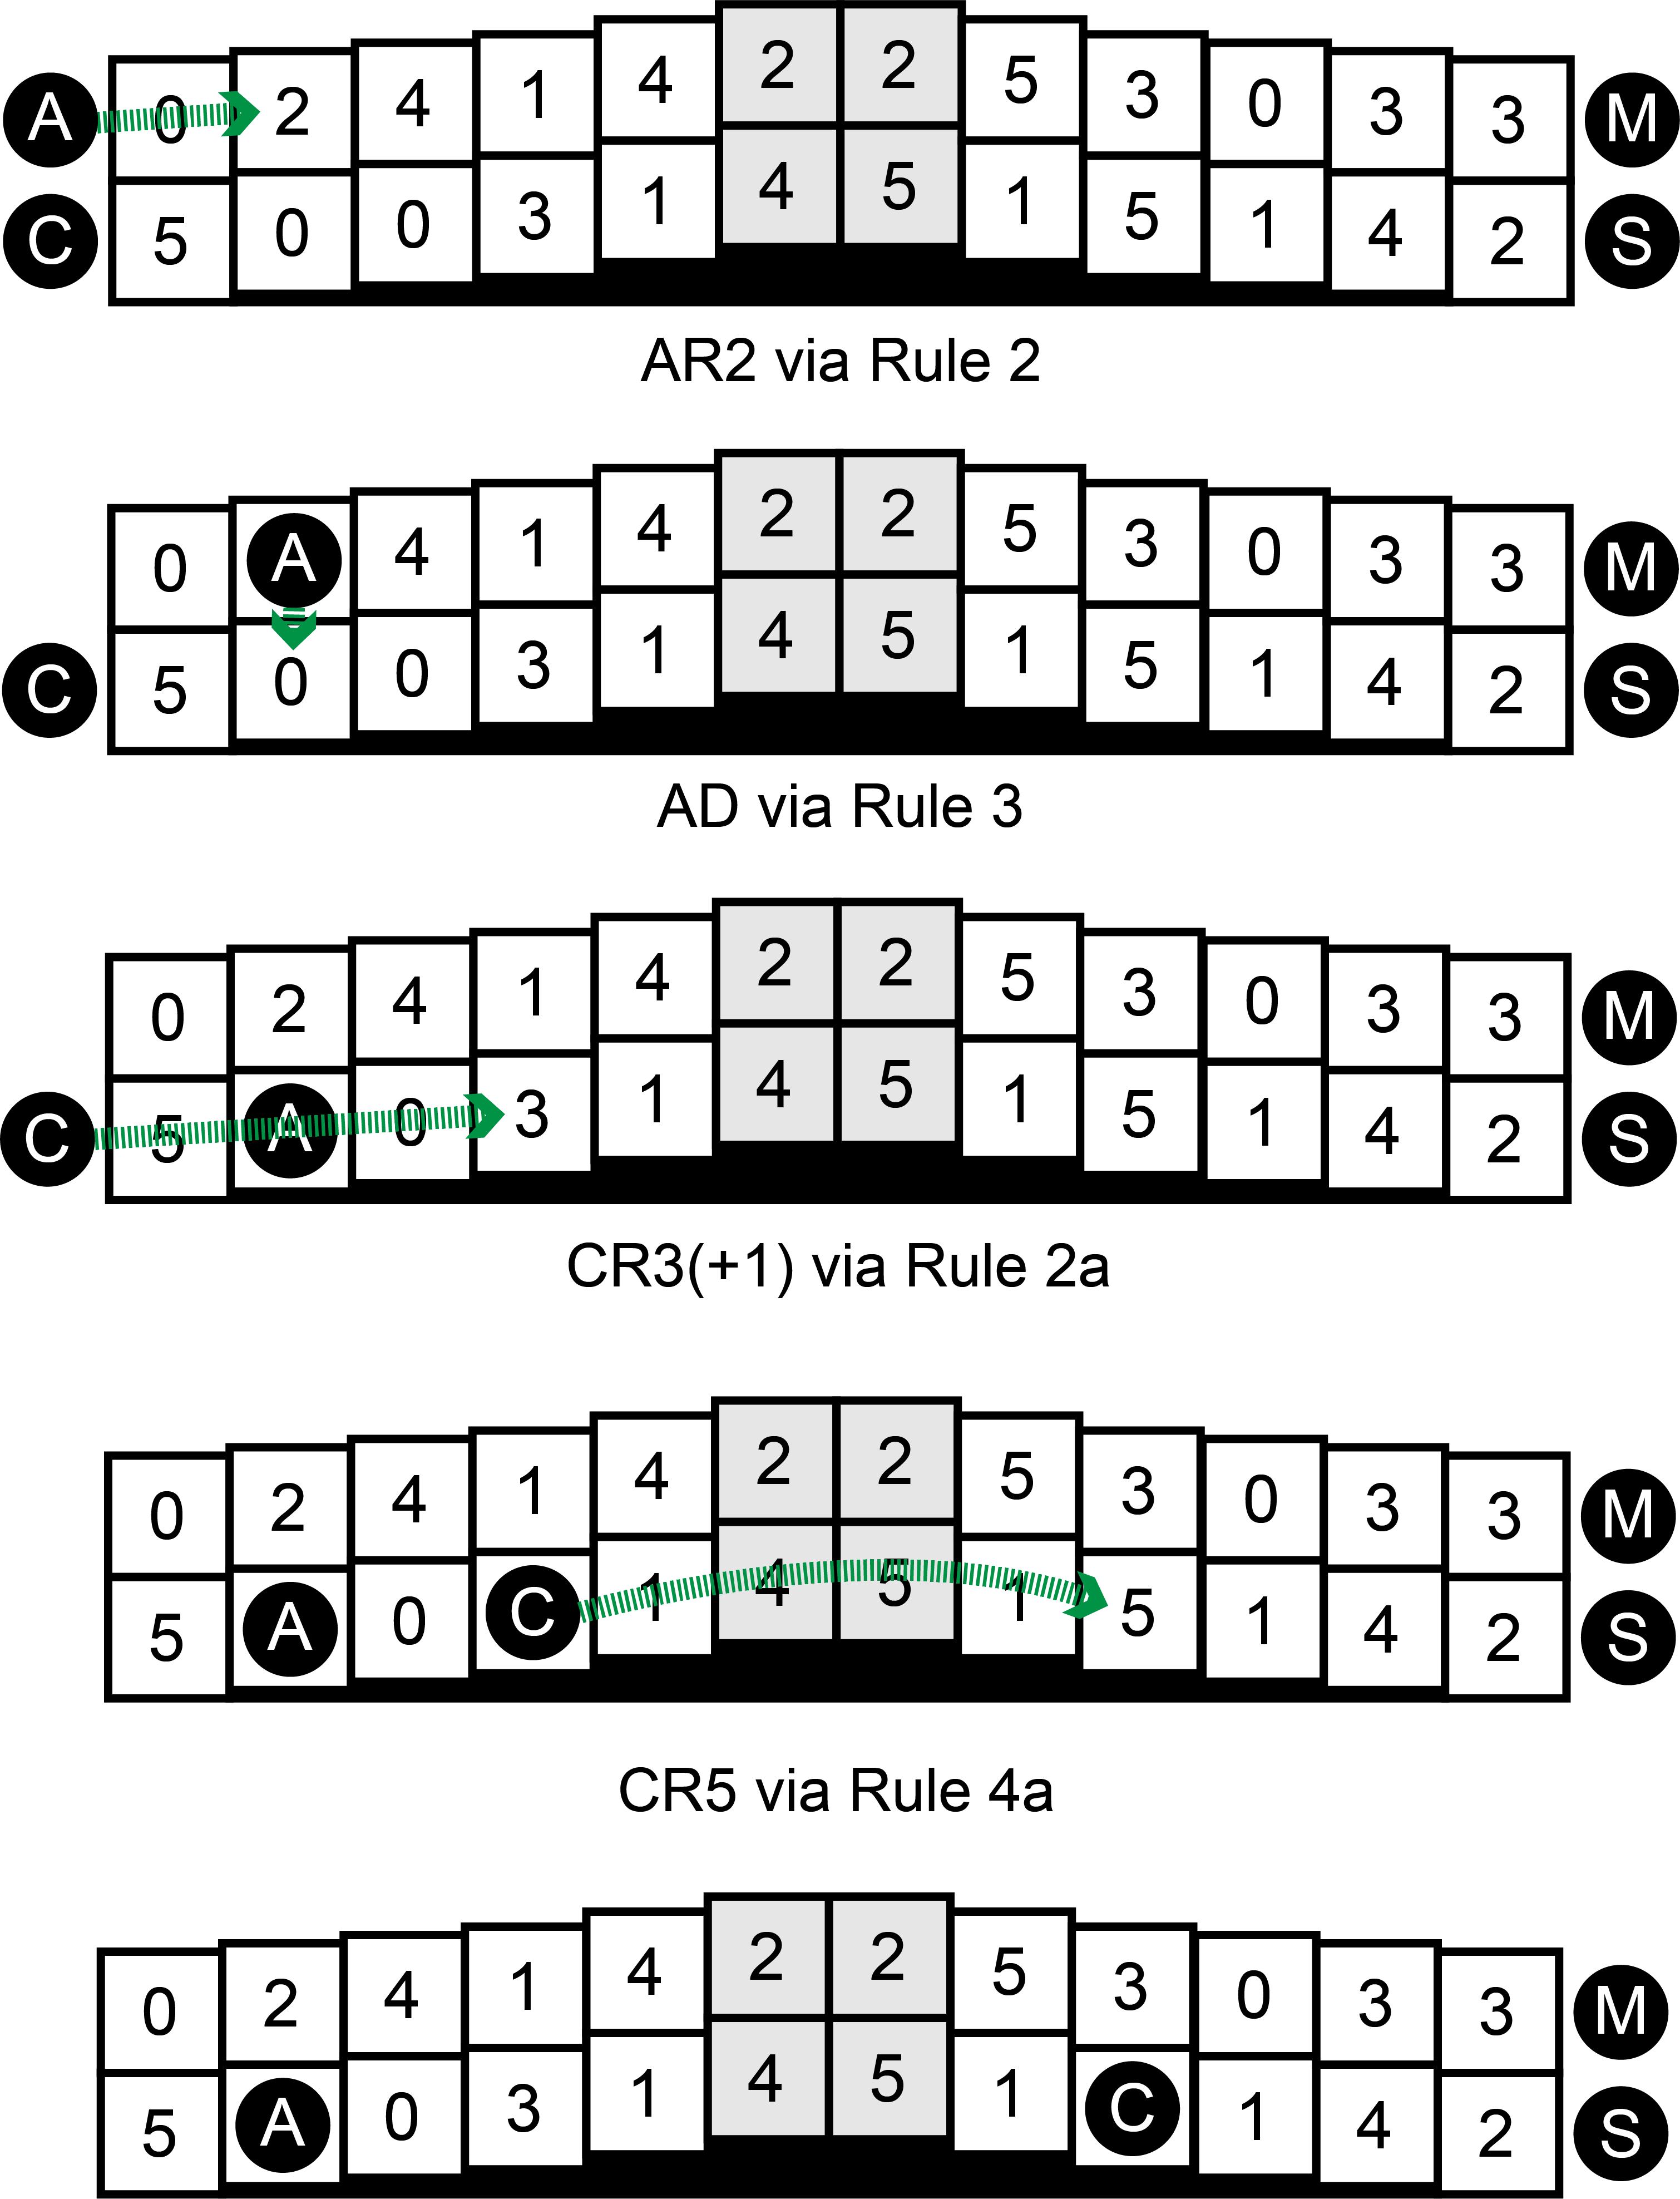
\includegraphics[width=8.8cm]{priestrulesfixed.png}
\caption{The start of a solution demonstrating the rules of Priest movement, with move notation followed by the matching rule. }
\label{fig:priestrules}
\end{figure}


There are, however, alternative PCG approaches available for physical solitaire games, most popularly demonstrated by the card game Klondike Solitaire. In particular, this game uses an {\it online, stochastic, generate-and-test} PCG algorithm, which is as simple as shuffling the deck of cards at the start of the game. Also of note, having a solution for Klondike is {\it optional}; the {\it test} portion of the generate-and-test algorithm is left to the solver as they play through the game. Wolter \cite{SOLITAIREVARIANTS} developed the Politaire system, and examines the effect of various shuffling algorithms across multiple solitaire card game variations. One variant called Thoughtful Solitaire, played such that all card locations are known to the solver at the beginning of the game, has been separately found to have setups between 82\% and 91.44\% solvable \cite{THOUGHTFUL}. Also falling within this classification is BoxOff, a 2D token removal puzzle, for which Browne and Maire investigated game parameters using Monte Carlo simulation \cite{MCPUZZLE}.
\noindent

%====================================================================================
\section{Fujisan} \label{section:fujisan}


To help us understand Fujisan challenge generation algorithms, we will first discuss the rules for solving Fujisan challenges, and the piecepack constraints that influenced its creation.

\subsection{Rules}
 \noindent
Functionally, the area of play consists of a grid of spaces arranged into two rows by twelve columns. Each space contains a single value in the range of 0 to 5, inclusive. The two middle columns together comprise the mountain {\it summit}, while each other column forms a {\it step} of the mountain. Four pawns, representing the Priests, start off the mountain, just outside the two columns furthest from the summit.

The goal of the solver is to {\bf move Priests one at a time until all four are at the summit.} A Priest can be moved according to the following rules:  

\begin{enumerate}
\item No more than one Priest may occupy a space at any given time.

\item A Priest may move onto a space if that space's value matches the number of unoccupied spaces the Priest must move in a straight line, left or right, to get there (including the destination space itself, but not including the Priest's starting space). %For example, a Priest may move onto a space containing a 4 if there are three unoccupied spaces between it and the Priest.
\begin{enumerate}
\item Occupied spaces (containing intervening Priests) are not counted when determining the distance from a Priest to a given space. %For example, a Priest may move onto a space containing a 2 if there are three occupied spaces and one unoccupied space between it and the Priest.
\end{enumerate}
\item A Priest may move freely up and down between the two spaces of any given step of the mountain. %This is the only manner in which a Priest may move onto a space containing a 0.
\begin{enumerate}
\item A Priest's first move from the starting position must land on the mountain; that is, the Priest cannot move up or down while on the ground.
\end{enumerate}

\item A Priest that lands on the mountain's summit can no longer move left or right, but may still move freely up or down within the column.\footnote{The original rules released for the piecepack version of Fujisan also allowed a Priest on the summit to freely move left and right, provided the Priest remained at the summit. The summit rule as written here was a change made for the Engraved Tiles version, and retained for the Dominoes version, both described in Section \ref{section:pcgalgs}. For purposes of statistical comparison, we have chosen to use this formulation of the rule for the computational simulations of all versions discussed.}
\begin{enumerate}
\item A Priest may pass over the summit as part of a move.
\end{enumerate}


\end{enumerate}

Figure \ref{fig:priestrules} shows a visual example of how these rules can be used to begin solving a sample challenge. We denote each move using a notation established by Kirkby\footnote{http://www.ludism.org/ppwiki/Fuji\_2dsan\_2fSolutionOne} where the Priest moving (A, C, M, or S) is followed by either U, D, L, or R, for Up, Down, Left, Right, respectively. On L and R moves, we include the unoccupied spaces traveled, with occupied spaces skipped shown in parentheses.


%====================================================================================
\subsection{Piecepack Components}

Fujisan was created specifically for the piecepack game system\footnote{http://www.ludism.org/ppwiki/SolitaryConfinement}. The piecepack is a set of board game parts that can be used to design and play a wide variety of games. The piecepack was designed and placed into the public domain in 2000. Figure \ref{fig:piecepackinfinite} shows one published version of the piecepack, including a rulebook of over 50 games that can be played with a piecepack.

Although several variations and ``expansions'' exist, a standard piecepack consists of the following components:
\begin{itemize}
\item 24 square tiles, indexed on the obverse in four suits (suns, moons, crowns, and arms) of six values each (null, ace, 2, 3, 4, and 5) and divided on the reverse into a 2$\times$2 space grid.
\item 24 round coins, each sized to fit comfortably into one space of a tile, marked on the obverse with one of the six values and on the reverse with one of the four suits.
\item 4 cubic dice, one per suit, each side marked with one of the six values.
\item 4 pawns, one per suit, each sized to fit comfortably into one space of a tile.
\end{itemize}

Fujisan uses the reverse side of 21 of the 24 tiles to form the mountain, the obverse of all 24 coins to assign values to spaces, and the four pawns to represent the Priests. Ace coins are assigned a value of 1, while null coins are assigned a value of 0. The dice are not used.

\begin{figure}[t]
\centering
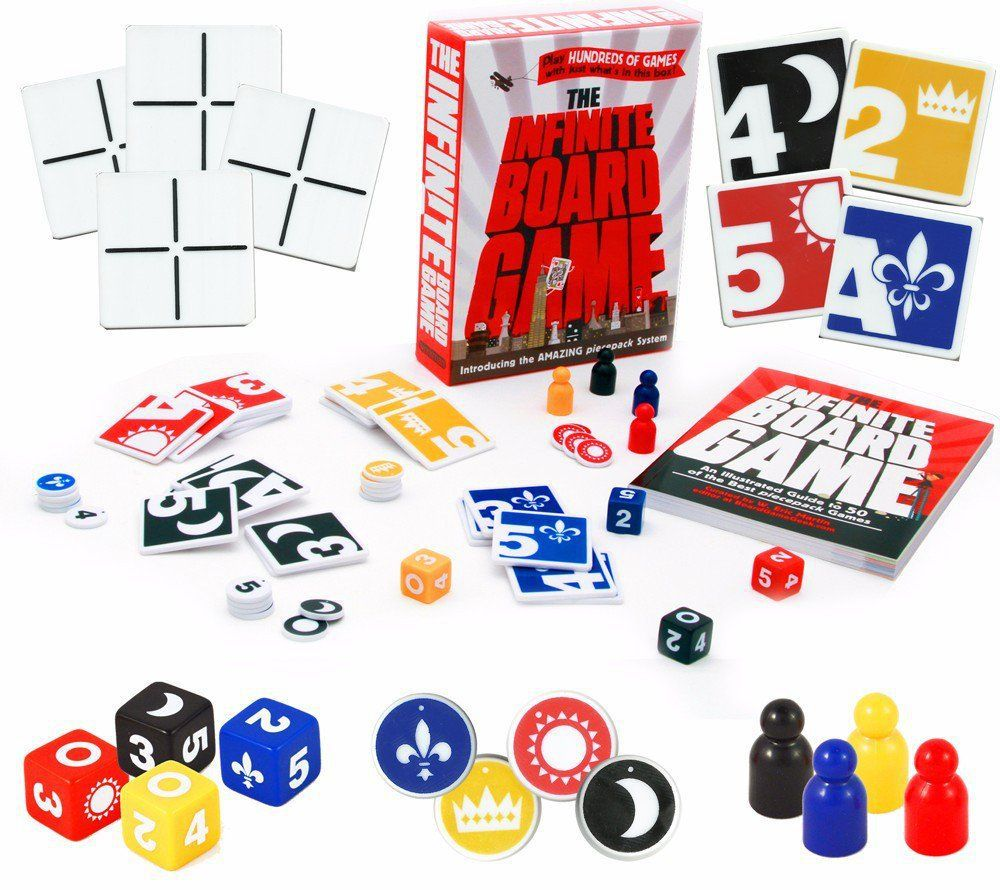
\includegraphics[width=7cm]{infinite2.jpg}
\caption{The piecepack, Infinite Board Game version. Photo courtesy of Workman
Publishing.}
\label{fig:piecepackinfinite}
\end{figure}

%====================================================================================
\section{PCG Setup Algorithms} \label{section:pcgalgs}

\noindent
Using the PCG taxonomy described in Section \ref{sec:Background}, Fujisan, like Klondike Solitaire, uses an {\it online, stochastic, generate-and-test, optional} PCG algorithm for challenge setup. However, if the solver reaches a point in Fujisan where progress toward a solution no longer appears to be made, it might not be obvious whether the challenge setup is indeed solvable. Fujisan's initial game state is preserved throughout play; the solver can easily return the Priests to their starting locations and begin the challenge anew at any time. Thus, it is important to find algorithms that maximize solvability.

Here we explore a progression of constraints that create multiple variant algorithms that can be used for physical online challenge setup for Fujisan. Important statistics about each algorithm are summarized in Table \ref{table_stats}, namely the number of possible challenges, the number of times a value may be repeated in a challenge, if the same value can occur in two spaces on the same step, and if the value pair present on a step can be repeated elsewhere in the challenge.

\begin{table*}[]
\centering
\renewcommand{\arraystretch}{1.3}
\caption{Statistics about Fujisan Setup Algorithms for each metric.}
\label{table_stats}
\begin{tabular}{l|c|c|c|c|}
\multicolumn{1}{c|}{\textbf{PCG}} & \multicolumn{1}{c|}{\textit{\textbf{Possible Challenges}}} & \multicolumn{1}{l|}{\textit{\textbf{Count of Each Value}}} & \multicolumn{1}{l|}{\textit{\textbf{Identical Step Values}}} & \multicolumn{1}{l|}{\textit{\textbf{Repeated Step Values}}} \\ \hline
\textbf{Random}                   & $10^{18}$                                  & 0 to 24                                                    & yes                                                      & yes                                                            \\ \hline
\textbf{Any Coin}                 & $10^{14}$ & exactly 4                                                  & yes                                                      & yes                                                            \\ \hline
\textbf{Piecepack}                & $10^{10}$                                             & exactly 4                                                  & no                                                       & yes                                                            \\ \hline
\textbf{Engraved}                 & $10^{13}$                                                 & 0 to 7$^*$                                                     & yes                                                      & only at summit                                                 \\ \hline
\textbf{Domino}                   & $10^{14} $                                                   & 2 to 5                                                     & no                                                       & no                                                             \\ \hline
\end{tabular}

\vspace{0.2cm} * 0 to 5 for value 0
\end{table*}

\subsection{Pure Random}

First, we examine a purely random process as a baseline algorithm for comparison purposes.

\begin{quote}
    
  Take one die from the piecepack. For each space, roll the die and place a coin that matches the number rolled on the space.
\end{quote}

With 24 spaces and six options for each space, this algorithm can generate $\frac{6^{24}}{4} \approx 10^{18}$ possible challenges. We divide by 4 here and in subsequent calculations to account for Fujisan challenges displaying rotational, horizontal, and vertical symmetry, however, this slightly underestimates due to some challenges displaying more than one symmetry. Each subsequent algorithm will constrain this randomness in some way, eliminating possible challenges from consideration.

\subsection{Any Coin}

Next, we examine two algorithms that make use of the piecepack coin components to generate randomness. These will constrain our solutions to have exactly four of each value.

\begin{quote}
    
  Shuffle the 24 coins face-down. For each space on the board, randomly select one coin and place it face-up on this space.
  
\end{quote}

Since each of the numbers 0 to 5 are present four times (once per suit), we can use the multinomial theorem to determine that this method can create
$\frac{24!}{4!^{6}4} \approx 10^{14}$ possible challenges. 

However, if two 0 coins are placed in same row, then it becomes impossible to move a Priest onto that row. This creates holes in our challenges and reduces the number of solvable setups. 
More importantly, when both spaces of either of the summit columns contain 0s, the challenge becomes impossible to solve.


\subsection{piecepack}

The original published Fujisan ruleset was devised to address the issue of double 0 steps, adding the constraint that each step must have two different values.

\begin{quote}
    
  Shuffle the 24 coins face-down, and separate into four groups based on their suit. Then repeatedly place two coins on the two right-most available spaces, choosing from each of the suits in turn (sun, moon, crown, arms).
\end{quote}


With each space limited to choosing from a particular suit, the piecepack algorithm will generate $\frac{6!^4}{4} \approx 10^{10}$ possible challenges. 
This algorithm will guarantee there are no double numbers on a step, thus eliminating the double 0 issue noted above. 

\subsection{Engraved Tiles}

\begin{figure}[t]
\centering
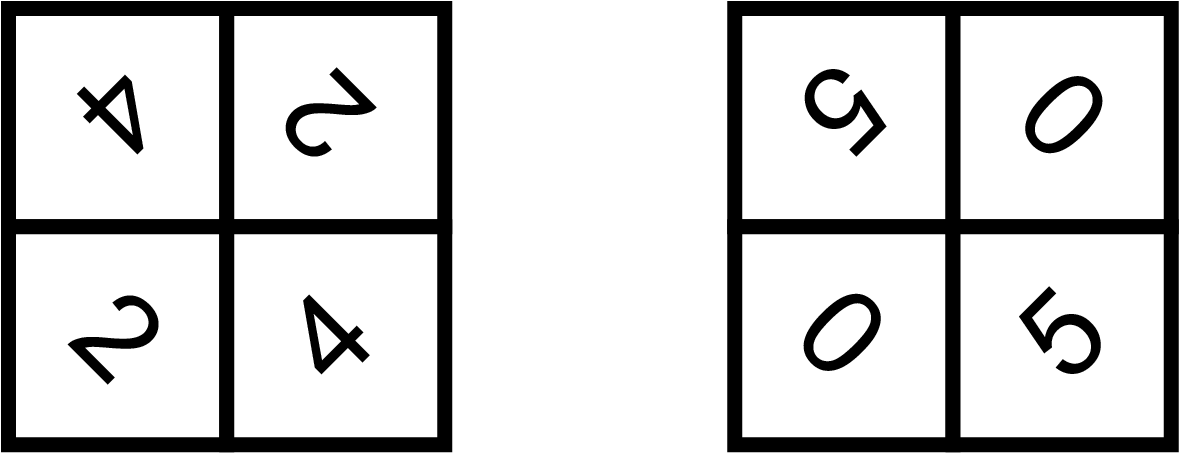
\includegraphics[width=4cm]{engravedsample.png}
\caption{Sample Engraved Fujisan Tiles.}
\label{fig:engravedsample}
\end{figure}


There are other ways to generate Fujisan challenges if we look beyond the original piecepack components. One option is to combine the values with the 2$\times$2 tiles, engraving
numerals onto the spaces. Here, we explore creating tiles with every possible pairing of values 0 through 5, including pairing a value with itself, and repeating these values diagonally on the tiles. Example tiles of this style are shown in Figure \ref{fig:engravedsample}. We remove the 0:0 pairing, since it can create unsolvable challenges, leaving 20 tiles.

\begin{quote}
    
  Shuffle the tiles face-down. Then, assemble the mountain by turning tiles face-up, using six for the bottom layer, five for the next layer, then four, then three, and finally two. The summit will be the center four spaces.
\end{quote}

This further constrains each pair of numbers to appear no more than once in the puzzle, except for the top two tiles. There are 20 possible tiles, and only 10 of them can be seen once the puzzle is constructed, as shown in Figure \ref{fig:tileexample}. 15 of these tiles have two possible orientations, for a total of $\sum_{i = 5}^{10}\frac{{15 \choose i}\binom{5}{10 - i}2^{i}10!}{4} \approx 10^{13}
$ possible challenges.

\begin{figure}[b]
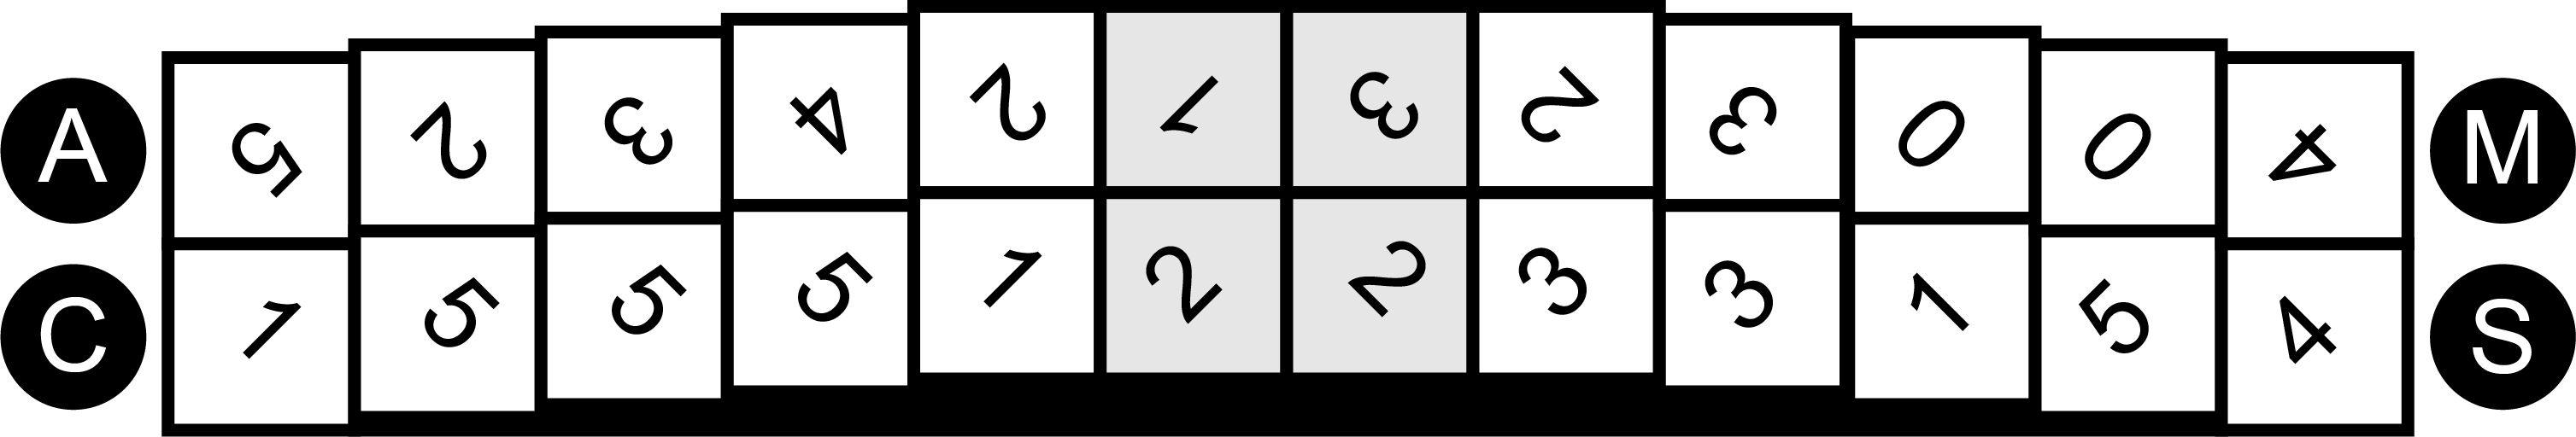
\includegraphics[width=8.8cm]{fujisan-engraved.png}
\caption{A sample Fujisan challenge from the Engraved Tiles algorithm.}
\label{fig:tileexample}
\end{figure}


\subsection{Dominoes}
Furthermore, we can look at alternate existing pieces with which to construct Fujisan challenges. A standard double-six domino set includes 28 dominoes. If we eliminate those dominoes that include a 6, along with all doubles, we are left with 15 dominoes. 

\begin{quote}
    
  Shuffle the dominoes face-down. Place 12 of these dominoes face-up in a row to create the mountain. Place a face-down domino on each side of the mountain to denote the starting locations for the Priests. Place the remaining face-down domino horizontally in the middle to raise up the two central dominoes, denoting the summit.
\end{quote}

This constraint is similar to the Engraved Tiles algorithm, but with a subset of the value pairs, thus a different probability on their selection.  Additionally, unlike the Engraved Tiles algorithm, the summit values are distinct from the two steps closest the summit.
With 15 possible dominoes, only 12 of them are used in the challenge, as shown in Figure \ref{fig:dominoexample}. Each of these dominoes has two possible orientations, for a total of $\frac{{15 \choose 12}2^{12}12!}{4} \approx 10^{14}$ possible challenges. 

\begin{figure}[b]
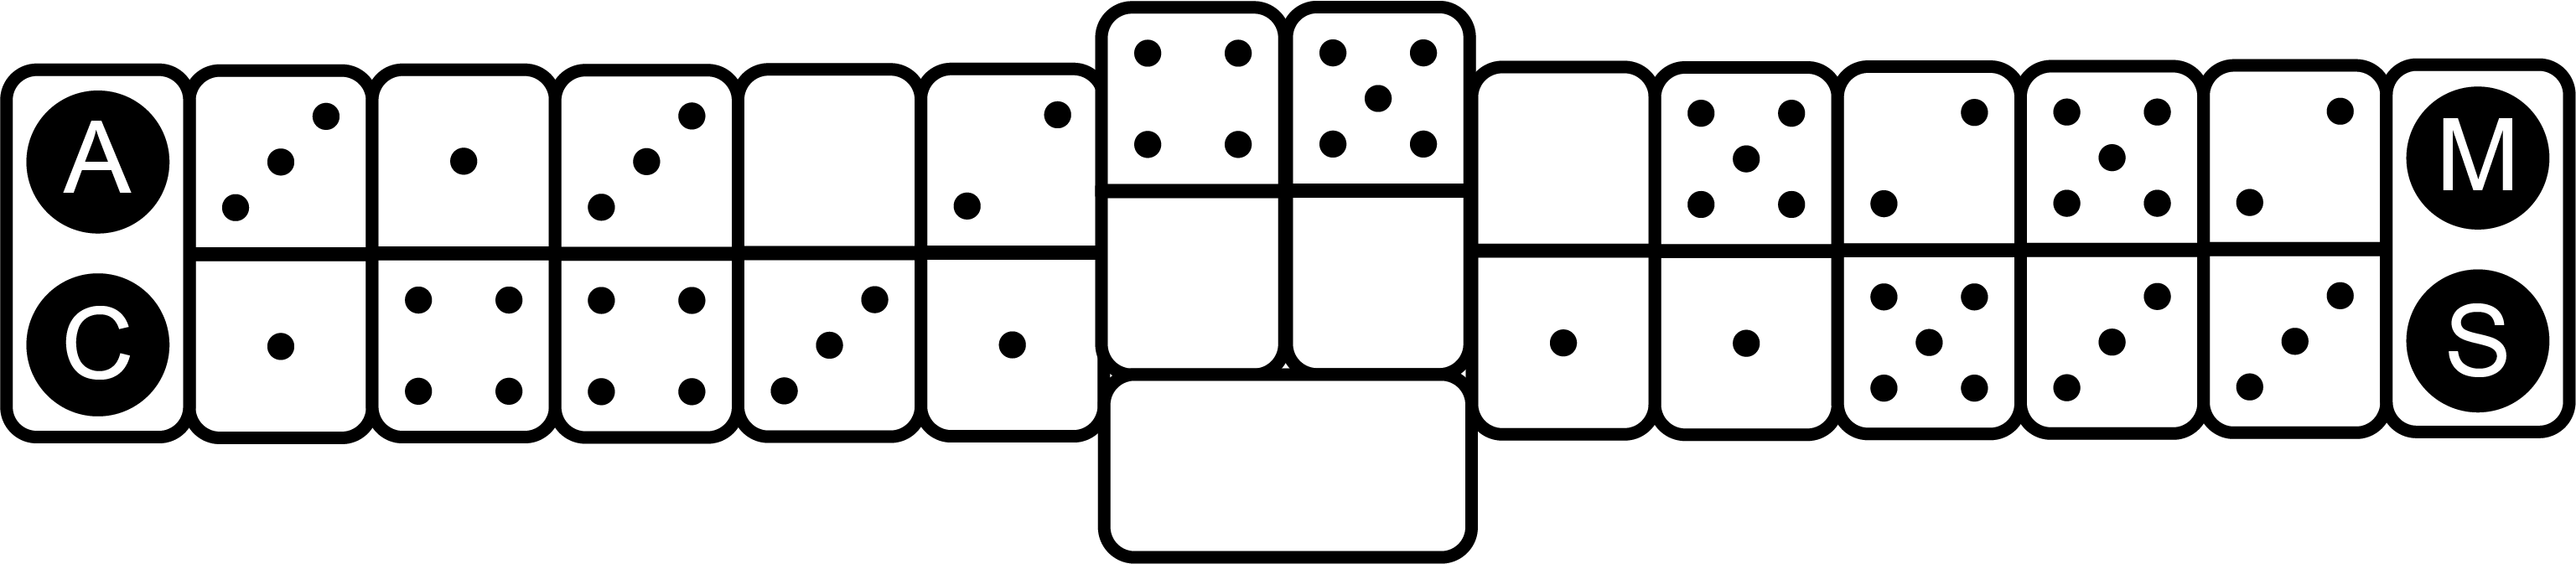
\includegraphics[width=8.8cm]{dominoexample.png}
\caption{A sample Fujisan challenge from the Dominoes algorithm.}
\label{fig:dominoexample}
\end{figure}



\section{Evaluation}

 \noindent
To evaluate each of the algorithms discussed above, we encoded a Monte Carlo Fujisan challenge generator using C\#, along with an A* solver for Fujisan challenges. Our admissible heuristic for A* is the number of empty spaces on the summit. For each PCG algorithm, we generated 1000 random challenges, divided into 10 trials of 100 challenges. 

We will use three criteria to quantify each of these variants:
{\bf ease of physical setup}, {\bf solvability}, and {\bf difficulty}.  First, our stochastic 
generation algorithm must be easy for the solver to execute without complicated lookup tables or large numbers of components. Next, we judge a PCG algorithm to be working well when a high percentage of generated games are solvable by our A* solver. Beyond solvability, we also wish for PCG algorithms to have a strong inclination to generate interesting and difficult challenges for the solver. 

For each generated challenge in our trials, we recorded if the challenge was solvable, and if so, we also recorded the minimum solution length found with our A* solver. The code used for our simulations is available on Github \footnote{http://github.com/mgoadric/fujisan}. 

\subsection{Ease of Physical Setup}

The {\bf Pure Random} algorithm rates very low on the ease of setup metric when considering the piecepack components. There could be many cases when a number was selected more than 4 times, thus exhausting the coins of one piecepack. Ultimately, six piecepacks would be needed for extreme cases when the same number is rolled for every space. Also, rolling a die 24 times at the beginning of a challenge quickly becomes tedious. 

{\bf Any Coin} is much more straightforward, since the coins can be shuffled on the table quickly, then added one by one to the board spaces. The {\bf piecepack} constraint, while equivalent in the number of actual coin placements, is a little more difficult to setup by the solver. Tracking the ordering of suits and following the pattern can slow down a solver setup, but this ordering can be quickly memorized on repeated play.

{\bf Engraved Tiles} shows a marked improvement in physical setup ease.
The numbers are already on the tiles, so the challenge is created in the process of building the mountain; no additional algorithm is needed. Likewise with {\bf Dominoes}, the challenge is again encoded in the board setup, and with fewer tiles, this setup is even more elegant.

\subsection{Solvability}

\begin{figure}[t]
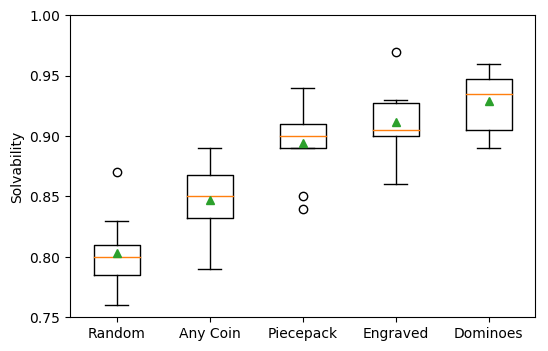
\includegraphics[width=8.8cm]{standalonesolve.png}
\caption{Effect of challenge generation algorithms on solvability.}
\label{fig:strategycomp}
\end{figure}

Figure \ref{fig:strategycomp} shows the distribution of solvability for the five PCG algorithms across the 10 trials in a box-and-whisker plot. The mean for each method is marked with a green triangle. Each method produces a healthy number of solvable challenges; every trial was above 75\% solvable. {\bf Pure Random} and {\bf Any Coin} have the lowest mean value for solvability and these results are significantly lower than the other three algorithms, which is confirmed by t-tests using a p-value of 0.05. 

Within the top three algorithms, only {\bf Dominoes} is statistically higher than {\bf piecepack}. To understand these results, we first explore the connections between steps in a challenge. We say step $A$ is connected to step $B$ in Fujisan if there is a move available according to rule 2 from $B$ to $A$. While critical to solving most challenges, we simplify our connectedness calculation by ignoring the impact of intermediate Priests between $B$ and $A$. 

Figure \ref{fig:connected} shows the average step connectedness within a challenge for each setup algorithm, differentiating solvable challenges in black from unsolvable challenges in white. We can see a large divide between solvable and unsolvable challenges on this metric for each algorithm, with higher connectivity always related to higher solvability. Also, as shown in Table \ref{table_stats}, both {\bf piecepack} and {\bf Dominoes} require that each step has two unique values. In these two algorithms, this uniqueness constraint strongly increases the connectedness of both solvable and unsolvable challenges, but the divide remains intact.

Second, for {\bf Engraved Tiles} and {\bf Dominoes}, repetition of pairs of values on a step are either restricted to the summit or not allowed elsewhere in the challenge. This causes the connections between steps to be more distributed and bind the puzzle together as a whole, instead of breaking apart into disjoint pieces. {\bf Dominoes} combines two constraints to create well-connected and well-distributed challenges.

\begin{figure}[t]
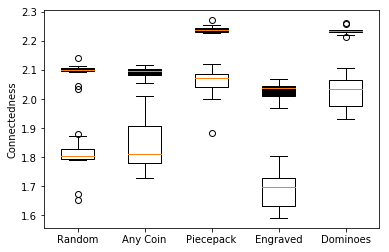
\includegraphics[width=8.8cm]{connectedness.png}
\caption{Average connectedness for Fujisan challenges across each setup algorithm. 
Solvable challenges shown in black, and unsolvable challenges shown in white.}
\label{fig:connected}
\end{figure}


\subsection{Difficulty}

Browne and Maire \cite{MCPUZZLE} propose a metric by which a solitaire game is interesting if the difference in solvability between an AI solver and a random solver is high. Across all of our PCG algorithms implemented for Fujisan, however, we found a random solver would win less than 0.3\%, making their metric equivalent to solvability for Fujisan. Instead, we define challenge difficulty here to be the minimum number of moves required to solve the challenge, and are interested in the distribution of challenge difficulties generated by each algorithm. We compare here the median level of challenge difficulty generated by each algorithm. The shortest possible solution to a Fujisan challenge involves eight moves, while 
the longest-known constructed challenge requires 62 moves\footnote{http://www.ludism.org/ppwiki/Fuji-san\#Heading9}.

\begin{figure}[t]
\centering
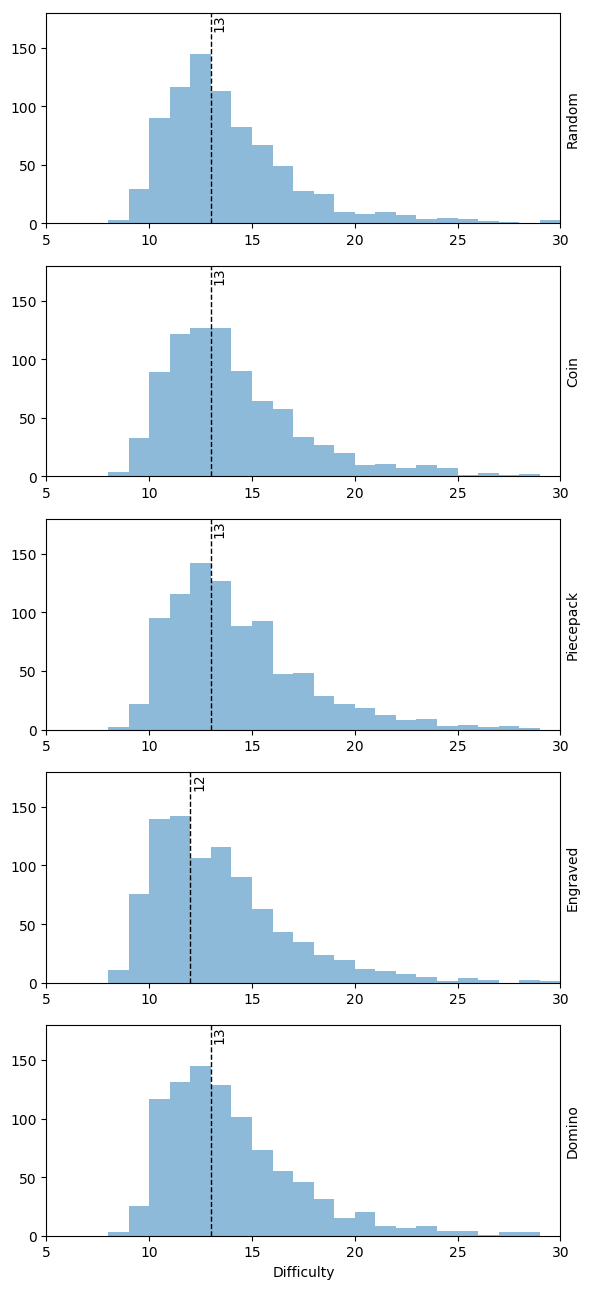
\includegraphics[width=8.5cm]{standalonediff.png}
\caption{Histograms showing the effect of challenge generation algorithms on difficulty.}
\label{fig:difficultycomp}
\end{figure}

Figure \ref{fig:difficultycomp} shows histograms of the minimum solution length for solvable challenges, pooled across all trials for each algorithm. The median is denoted with a dotted line. Our algorithms appear to follow a Poisson distribution rather than a normal distribution, since the smallest possible solution length for any challenge is 8, and the maximum solution length is currently unbounded. We employ a Kruskal-Wallis H-test \cite{KRUSKAL} to determine if the median difficulty of our five algorithms is statistically the same, and we reject this null hypothesis very strongly, with a p-value of $1.9 \times 10^{-8}$.

The algorithm responsible for this result is {\bf Engraved Tiles}. We can see a strong tendency to have shorter solution lengths, with almost 10\% of challenges having a solution length of eight or nine, whereas for {\bf Dominoes}, this is true for only 3\% of challenges. In {\bf Engraved Tiles}, there are five tiles that contain a 0 value; since there will be ten total tiles hidden, on average a challenge will contain 2.5 zeros values. It appears that 0 values are one part of what makes Fujisan challenges interesting, since having fewer 0 values decreases the challenge difficulty.


\subsection{Summary}
\begin{table}[]
\centering
\renewcommand{\arraystretch}{1.3}
\caption{Ranks of Fujisan Setup Algorithms for each metric.\\ Statistical ties are denoted with *.}
\label{table_example}
\begin{tabular}{l|c|c|c|}
\multicolumn{1}{c|}{\textbf{PCG}} & \multicolumn{1}{l|}{\textit{\textbf{Setup}}} & \multicolumn{1}{l|}{\textit{\textbf{Solvability}}} & \multicolumn{1}{l|}{\textit{\textbf{Difficulty}}} \\ \hline
\textbf{Random}                   & 5                                            & 5                                                  & 1*                                                 \\ \hline
\textbf{Any Coin}                 & 3                                            & 4                                                  & 1*                                                 \\ \hline
\textbf{Piecepack}                & 4                                            & 2*                                                  & 1*                                                 \\ \hline
\textbf{Engraved}                 & 2                                            & 2*                                                  & 5                                                 \\ \hline
\textbf{Domino}                   & 1                                            & 1                                                  & 1*                                                 \\ \hline
\end{tabular}
\end{table}

Table \ref{table_example} summarizes our results on the three evaluation metrics. We can see computational evidence that the original {\bf piecepack} ruleset is an improvement over both the {\bf Pure Random} and {\bf Any Coin} setup algorithm as hoped by the designer. While {\bf Engraved Tiles} simplifies the ease of physical setup over the {\bf piecepack} version, it is at the cost of challenge difficulty. The {\bf Dominoes} algorithm maintains this easy setup and returns the challenge generation to a reasonable difficulty distribution.


%====================================================================================

\section{Conclusion}   \label{sec:Conclusion}

\noindent
Our work helps frame puzzle generation, particularly within solitaire puzzle games, within the taxonomy of procedural content generation (PCG). By examining variants for challenge creation, we can see that subtle changes in the random distribution used in an algorithm can have large-scale changes on the generated content.

There are many open questions related to physical games and PCG. First, we believe there is work to be done in formalizing our ease of physical setup metric. A simple approximation would be the time complexity of the algorithm, however, certain operations that are straightforward to a computer can be difficult for humans to track, and vice versa. With a formal metric, game and puzzle designers could be inclined to include more intricate PCG algorithms in their designs when provided guarantees these algorithms can reasonably be executed by a human player.

A further point to clarify is the exact relationship between the minimum solution length and challenge difficulty. We believe this metric can be expanded to include the branching factor along the solution path. Also, we have ignored a difference in move clarity for Fujisan. Up and down moves are always available for Priests on the mountain, but left and right moves must be visually identified and recalculated as spaces become occupied. It is unclear, therefore, whether both types of movement contribute equally to the level of challenge experienced by the solver. A more sophisticated difficulty metric could take these into account and further differentiate the above setup algorithms.

Finally, are there general methods that allow solvers to {\it construct} challenges online to guarantee solvability, as opposed to the {\it generate-and-test} algorithms discussed here? While this may be possible in certain situations, as employed in another piecepack solitaire game Cell Management \footnote{http://www.ludism.org/ppwiki/CellManagement}, care must be taken that the construction process does not give away the solution to the challenge.


%====================================================================================

%\section*{Acknowledgements}

%\noindent
%Thanks to XYZ and the anonymous reviewers for their helpful and insightful comments.

%====================================================================================

% An example of a floating figure using the graphicx package.
% Note that \label must occur AFTER (or within) \caption.
% For figures, \caption should occur after the \includegraphics.
% Note that IEEEtran v1.7 and later has special internal code that
% is designed to preserve the operation of \label within \caption
% even when the captionsoff option is in effect. However, because
% of issues like this, it may be the safest practice to put all your
% \label just after \caption rather than within \caption{}.
%
% Reminder: the "draftcls" or "draftclsnofoot", not "draft", class
% option should be used if it is desired that the figures are to be
% displayed while in draft mode.
%
%\begin{figure}[!t]
%\centering
%\includegraphics[width=2.5in]{myfigure}
% where an .eps filename suffix will be assumed under latex, 
% and a .pdf suffix will be assumed for pdflatex; or what has been declared
% via \DeclareGraphicsExtensions.
%\caption{Simulation results for the network.}
%\label{fig_sim}
%\end{figure}

% Note that the IEEE typically puts floats only at the top, even when this
% results in a large percentage of a column being occupied by floats.
% However, the Computer Society has been known to put floats at the bottom.


% An example of a double column floating figure using two subfigures.
% (The subfig.sty package must be loaded for this to work.)
% The subfigure \label commands are set within each subfloat command,
% and the \label for the overall figure must come after \caption.
% \hfil is used as a separator to get equal spacing.
% Watch out that the combined width of all the subfigures on a 
% line do not exceed the text width or a line break will occur.
%
%\begin{figure*}[!t]
%\centering
%\subfloat[Case I]{\includegraphics[width=2.5in]{box}%
%\label{fig_first_case}}
%\hfil
%\subfloat[Case II]{\includegraphics[width=2.5in]{box}%
%\label{fig_second_case}}
%\caption{Simulation results for the network.}
%\label{fig_sim}
%\end{figure*}
%
% Note that often IEEE papers with subfigures do not employ subfigure
% captions (using the optional argument to \subfloat[]), but instead will
% reference/describe all of them (a), (b), etc., within the main caption.
% Be aware that for subfig.sty to generate the (a), (b), etc., subfigure
% labels, the optional argument to \subfloat must be present. If a
% subcaption is not desired, just leave its contents blank,
% e.g., \subfloat[].


% An example of a floating table. Note that, for IEEE style tables, the
% \caption command should come BEFORE the table and, given that table
% captions serve much like titles, are usually capitalized except for words
% such as a, an, and, as, at, but, by, for, in, nor, of, on, or, the, to
% and up, which are usually not capitalized unless they are the first or
% last word of the caption. Table text will default to \footnotesize as
% the IEEE normally uses this smaller font for tables.
% The \label must come after \caption as always.
%
%\begin{table}[!t]
%% increase table row spacing, adjust to taste
%\renewcommand{\arraystretch}{1.3}
% if using array.sty, it might be a good idea to tweak the value of
% \extrarowheight as needed to properly center the text within the cells
%\caption{An Example of a Table}
%\label{table_example}
%\centering
%% Some packages, such as MDW tools, offer better commands for making tables
%% than the plain LaTeX2e tabular which is used here.
%\begin{tabular}{|c||c|}
%\hline
%One & Two\\
%\hline
%Three & Four\\
%\hline
%\end{tabular}
%\end{table}


% Note that the IEEE does not put floats in the very first column
% - or typically anywhere on the first page for that matter. Also,
% in-text middle ("here") positioning is typically not used, but it
% is allowed and encouraged for Computer Society conferences (but
% not Computer Society journals). Most IEEE journals/conferences use
% top floats exclusively. 
% Note that, LaTeX2e, unlike IEEE journals/conferences, places
% footnotes above bottom floats. This can be corrected via the
% \fnbelowfloat command of the stfloats package.


% if have a single appendix:
%\appendix[Proof of the Zonklar Equations]
% or
%\appendix  % for no appendix heading
% do not use \section anymore after \appendix, only \section*
% is possibly needed

% use appendices with more than one appendix
% then use \section to start each appendix
% you must declare a \section before using any
% \subsection or using \label (\appendices by itself
% starts a section numbered zero.)
%


% Can use something like this to put references on a page
% by themselves when using endfloat and the captionsoff option.
\ifCLASSOPTIONcaptionsoff
  \newpage
\fi



% trigger a \newpage just before the given reference
% number - used to balance the columns on the last page
% adjust value as needed - may need to be readjusted if
% the document is modified later
%\IEEEtriggeratref{8}
% The "triggered" command can be changed if desired:
%\IEEEtriggercmd{\enlargethispage{-5in}}

% references section

% can use a bibliography generated by BibTeX as a .bbl file
% BibTeX documentation can be easily obtained at:
% http://mirror.ctan.org/biblio/bibtex/contrib/doc/
% The IEEEtran BibTeX style support page is at:
% http://www.michaelshell.org/tex/ieeetran/bibtex/
\bibliographystyle{IEEEtran}
% argument is your BibTeX string definitions and bibliography database(s)
\bibliography{references.bib}
%
% <OR> manually copy in the resultant .bbl file
% set second argument of \begin to the number of references
% (used to reserve space for the reference number labels box)
%\begin{thebibliography}{4}

%\bibitem{NONOGRAM} Batenburg, K. J., Henstra, S., Kosters, W. A., and  Palenstijn, W. J. `Constructing simple nonograms of varying difficulty.' {\it Pure Mathematics and Applications (Pu. MA)} 20 (2009): 1-15.

%\bibitem{THOUGHTFUL} Bjarnason, R., Tadepalli, P., and Fern, A. `Searching Solitaire in Real Time.' {\it ICGA Journal} 30.3 (2007): 131-142.

%\bibitem{KLONDIKEPLANNING} Bjarnason, R., Fern, A., and Tadepalli, P. `Lower Bounding Klondike Solitaire with Monte-Carlo Planning.' {\it ICAPS}. (2009).

%\bibitem{PUZZLENATURE} Browne, C., `The Nature of Puzzles', {\it Game and Puzzle Design}, vol. 1, no. 1, (2015), pp. 23-24.

%\bibitem{PCGSURVEY} Hendrikx, M., Meijer, S., Van Der Velden, J., and Iosup, A. `Procedural content generation for games: A survey.' {\it ACM Transactions on Multimedia Computing, Communications, and Applications (TOMM)} 9.1 (2013): 1.

%\bibitem{SUDOKU} Hunt, M.,  Pong, C. and Tucker, G, `Difficulty-Driven Sudoku Puzzle Generation' {\it The UMAP Journal} 29 (3) (2008) 343–362.

%\bibitem{FIFTEEN} Karlemo, F. R., and R. J. Patric. `On sliding block puzzles.' {\it Methods} 13.14 (2000): 15.

%\bibitem{TANGRAM} K{\"o}pp, W. `Random Generation of Tangrams.' Interdisciplinary Project in Mathematics, Technische Universitat M{\"u}nchen. (2015)

%\bibitem{KRUSKAL} Kruskal, W. H.,  and Wallis, W. W. `Use of Ranks in One-Criterion Variance Analysis', {\it Journal of the American Statistical Association}, Vol. 47, Issue 260, pp. 583-621, (1952).

%\bibitem{GAMESYSTEM} Kyle, J. `The piecepack: In Search of a Generic, Universal Boardgame Set' {\it Grampa Barmo's Discount Game Magazine} \#1 (2001)

%\bibitem{SBPCG} Togelius, J., Yannakakis, G., Stanley, K., and Browne, C. (2011). `Search-Based Procedural Content Generation: A Taxonomy and Survey'. {\it Computational Intelligence and AI in Games, IEEE Transactions on.} 3. 172 - 186.

%\bibitem{PEG} Uehara, R., and Shigeki I. `Generalized Hi-Q is NP-complete.' {\it IEICE TRANSACTIONS (1976-1990)} 73.2 (1990): 270-273.

%\bibitem{RUSHHOUR} van Dijk, Jelle. `Performance optimization of Rush Hour board generation.' Bachelors Thesis, University of Amsterdam (2018).

%\bibitem{SOLITAIREVARIANTS} Wolter, J. `Experimental Analysis of
%Various Solitaire Games' (2013) https://politaire.com/article/intro.html

%\end{thebibliography}
% biography section
% 
% If you have an EPS/PDF photo (graphicx package needed) extra braces are
% needed around the contents of the optional argument to biography to prevent
% the LaTeX parser from getting confused when it sees the complicated
% \includegraphics command within an optional argument. (You could create
% your own custom macro containing the \includegraphics command to make things
% simpler here.)
%\begin{IEEEbiography}[{\includegraphics[width=1in,height=1.25in,clip,keepaspectratio]{mshell}}]{Michael Shell}
% or if you just want to reserve a space for a photo:
\newpage 

\begin{IEEEbiography}[{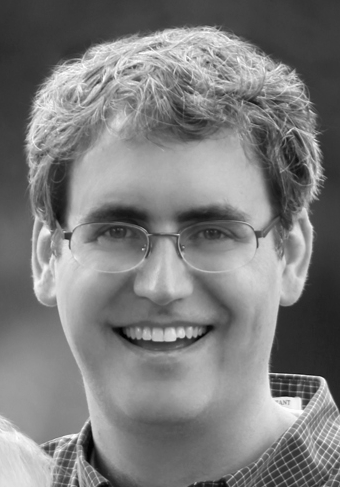
\includegraphics[width=1in,height=1.25in,clip,keepaspectratio]{markpic.png}}]{Mark Goadrich} earned an A.B. in Mathematics and Philosophy at Kenyon College, and a M.S. and Ph.D. in Computer Sciences from the University of Wisconsin - Madison.
He is currently an Associate Professor of Computer Science at Hendrix College in Conway, AR.
\end{IEEEbiography}

% if you will not have a photo at all:
\begin{IEEEbiography}[{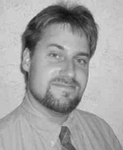
\includegraphics[width=1in,height=1.25in,clip,keepaspectratio]{jamespic.png}}]{James Droscha}
is a designer and developer of software, games, and puzzles, including the piecepack and Fujisan.
\end{IEEEbiography}

% insert where needed to balance the two columns on the last page with
% biographies
%\newpage

% You can push biographies down or up by placing
% a \vfill before or after them. The appropriate
% use of \vfill depends on what kind of text is
% on the last page and whether or not the columns
% are being equalized.

\vfill

% Can be used to pull up biographies so that the bottom of the last one
% is flush with the other column.
%\enlargethispage{-5in}



% that's all folks
\end{document}


